\section{GoCD}
    Systém GoCD vychází z projektu Cruise \cite{thoughtworks-gocd}. Oba projekty vznikly ve firmě ThoughtWorks, kde pracoval průkopník a zastánce praktik \textit{extrémního programování} M. Fowler \cite{fowler-go}. Fowler systém Cruise doporučoval ve známém článku o \CI \cite{fowler-ci}.

    \subsection{Architektura GoCD, možnosti konfigurace}
        GoCD stejně jako většina ostatních \CI staví na architektuře jednoho kontrolního serveru a řadě interních nebo externích agentů, které se starají o spuštění jednotlivých jobů. Ve výchozím nastavení jsou data persistována v embedované H2 databázi na server procesu. Instalace GoCD je díky tomu jednoduchá, protože stačí zaregistrovat externí repozitář a nainstalovat balíček pro server a pro agenty.

        Po prvním zobrazení webového rozhraní serveru se zobrazuje quick-start, který provádí vytvořením nové pipeline. Přestože GoCD podporuje \textit{Pipelines as code}, očekávaný primární vstup je klikání v administraci \cite{gocd-pas}. Načítání externích souborů je vyřešeno rozšířením, jehož použití se definuje v hlavní \glstext{XML} konfiguraci na webu. Separovaná konfigurace tak není kompletní a závisí na další ruční konfiguraci.

    \subsection{Rozšiřitelnost}
        GoCD nabízí několik možností, jak rozšiřovat výchozí funkcionalitu pomocí pluginů \cite{gocd-extensions}. Na rozdíl od Jenkins, kde lze upravit prakticky cokoliv, vystavuje pro pluginy GoCD jenom některá \glstext{API}. Nelze tak například ovlivňovat uživatelské rozhraní.

        Zhruba 80 pluginů je na oficiálním registru \cite{gocd-plugins}. ThoughtWorks~Inc.~zaštiťují 8 pluginů a a z toho je 6 placených.

        Z veřejně dostupných rozšíření jsou všechna kromě jednoho hostována na GitHub. Jak jsem ale vizualizoval \pfxref{v  grafu}{fig:jenkins-plugins}, GoCD rozšíření jsou ještě hůř udržovaná než ta pro Jenkins. A to je jich méně než dvacetina.

        \begin{iffigure}
            \centering
            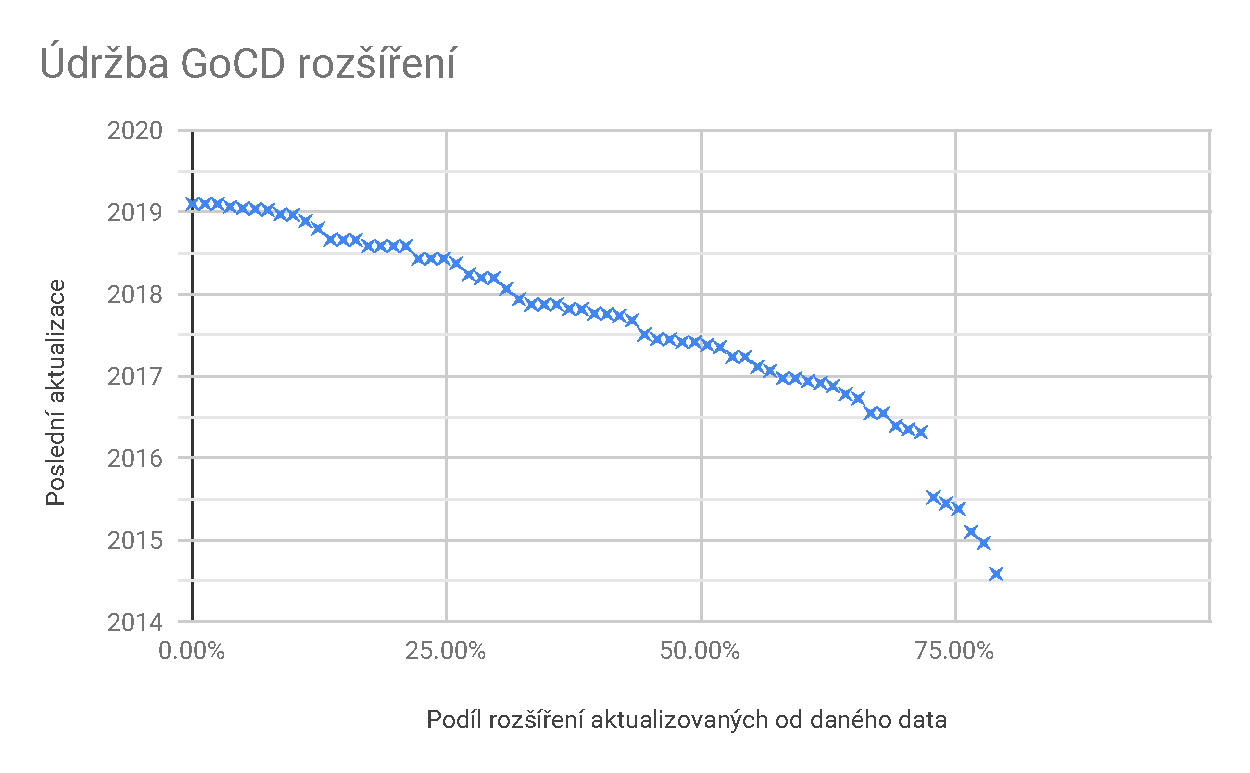
\includegraphics[width=\textwidth,height=9cm,keepaspectratio]{media/go-plugins-update.pdf}
            \caption{Rozdělení podle poslední aktualizace. Pouze 17 rozšíření (20 \%) bylo aktualizováno v posledním půl roce. Pouhých 30~\% rožšíření mělo alespoň jednu aktualizaci za poslední rok. Přibližně 20 \% rozšíření nemá žádné stabilní vydání. Zdroj: data vytěžena z GitHub repozitářů, dostupná na přiloženém mediu v \code{appendix/gocd-plugins.csv}.}
            \label{fig:jenkins-plugins}
        \end{iffigure}

    \subsection{Zabezpečení}
        Po instalaci serveru je v základu celá administrace dostupná pro všechny, bez autorizace. Lze zapnout zabudovaná rozšíření, která zprovozní přihlášení heslem a nebo přes \glstext{LDAP}. Nic v \glstext{UI} k tomu ale správce nenabádá. Velmi překvapivě ale není v Shodan databázi žádná nezabezpečená instance GoCD na výchozím portu \cite{shodan-gocd}.

        Izolace klientů závisí na použítých agentech. Klasický agent používá sdílené prostředí a zdroje, ale GoCD podporuje tzv.~\textit{Elastic Agent}, které se zapínají a vypínají dynamicky podle poptávky. Lze je využít pro zapnutí nového prostředí v Dockeru, Kubernetes, OpenStacku a několika dalších. Tato jednorázová prostředí nabízí lepší izolaci. Nenašel jsem rozšíření, které by dokázalo spravovat Elastic Agents pro VMware nebo jiný virtualizační nástroj, který by měl ještě lepší izolaci klientů.

        Na webu \glstext{CVE} Details jsem pro GoCD nenašel žádná historická \glstext{CVE}. Projekt ale využívá platformu HackerOne, kde za poslední tři roky zpracovali 39 nahlášených chyb \cite{gocd-hackerone}. Ze zveřejněných reportů je vidět, že správci reagují rychle a bezpečnostní chyby opravují v co nejkratším možném termínu.

    \subsection{Dostupnost}
        GoCD agenti jsou z principu stavové aplikace a stejně jako u všech ostatních \CI jejich výpadek přijdeme o spuštěné joby. Může jich ale běžet mnoho a pomocí rolling update je lze aktualizovat bez výpadku.

        Server je bohužel také stavový a může běžet pouze v jedné replice. GoCD prodává velmi drahý \textit{Business Continuity Addon}, který dokáže udržovat standby repliku \cite{gocd-ha}. Failover proces ale není nijak automatizovaný a povýšení na primární repliku vyžaduje restart GoCD serveru. U GoCD nelze udělat perfektní HA bez ztráty žádnéoho requestu když vypadne primární replika.

        \todo{Jak se dělá upgrade? Jak stabilní to je?}\blind[1]

    \subsection{Integrace}
        \todo{Integrace GoCD, oznámení na GitHub/GitLab/Bitbucket/\ldots}\blind[2]
        \todo{Možnosti deploy z GoCD do cílového systému; k8s, sftp, openstack, \ldots}\blind[5]

    \subsection{Praktické nasazení projektů}
        \subsubsection{Projekt 1}
            \todo{ze jsem bojoval s env, jinak vlastne v pohode, prirovanat k jenkins}
            \todo{Popsat deploy projektu 1 z GoCD}\blind[2]

        \subsubsection{Projekt 2}
            \todo{Popsat deploy projektu 2 z GoCD}\blind[2]

        \subsubsection{Projekt 3}
            \todo{Popsat deploy projektu 3 z GoCD}\blind[2]
